% Compile with pdfLaTeX, from project root. Independent of main.tex.
\documentclass[aspectratio=169,11pt]{beamer}
\usepackage[T1]{fontenc}
\usepackage{lmodern,booktabs,amsmath,graphicx,tikz}
\usetikzlibrary{positioning,arrows.meta}
\definecolor{navy}{HTML}{173653}
\definecolor{teal}{HTML}{007E80}
\definecolor{muted}{HTML}{526A7D}
\definecolor{pale}{HTML}{EDF3F6}
\definecolor{red}{HTML}{AE463D}
\setbeamercolor{normal text}{fg=navy,bg=white}
\setbeamercolor{frametitle}{fg=white,bg=navy}
\setbeamercolor{structure}{fg=teal}
\setbeamercolor{block title}{fg=white,bg=navy}
\setbeamercolor{block body}{fg=navy,bg=pale}
\setbeamercolor{alerted text}{fg=red}
\setbeamertemplate{navigation symbols}{}
\setbeamertemplate{itemize item}{\color{teal}\small$\blacktriangleright$}
\setbeamertemplate{frametitle}{\nointerlineskip\begin{beamercolorbox}[wd=\paperwidth,ht=0.86cm,dp=.22cm,leftskip=.55cm,rightskip=.3cm]{frametitle}\large\bfseries\insertframetitle\end{beamercolorbox}}
\setbeamertemplate{footline}{\leavevmode\hbox{\begin{beamercolorbox}[wd=.88\paperwidth,ht=.28cm,dp=.16cm,leftskip=.55cm]{normal text}\scriptsize\color{muted}DTU Compute \hspace{.25cm}$|$\hspace{.25cm} MSc thesis defense\end{beamercolorbox}\begin{beamercolorbox}[wd=.12\paperwidth,ht=.28cm,dp=.16cm,rightskip=.5cm plus1fil]{normal text}\scriptsize\hfill\insertframenumber\end{beamercolorbox}}}
\setbeamersize{text margin left=.55cm,text margin right=.55cm}
\newcommand{\key}[1]{\textcolor{teal}{\textbf{#1}}}
\newcommand{\smallnote}[1]{\par\vspace{.12cm}{\scriptsize\color{muted}#1}}
\newcommand{\fig}[2]{%
\IfFileExists{Backmatter/unified_#2.pdf}{\includegraphics[width=\linewidth,height=#1,keepaspectratio]{Backmatter/unified_#2.pdf}}{%
\IfFileExists{reports/publication_assets/figures/#2.pdf}{\includegraphics[width=\linewidth,height=#1,keepaspectratio]{reports/publication_assets/figures/#2.pdf}}{\includegraphics[width=\linewidth,height=#1,keepaspectratio]{../reports/publication_assets/figures/#2.pdf}}}}
\newcommand{\take}[1]{\begin{block}{Takeaway}#1\end{block}}
\title{Vision Foundation Models for Industrial Anomaly Detection}
\subtitle{Robustness and Reference Augmentation in One-Shot Learning}
\author{Bashar Khaled Bdewi}
\institute{MSc Human-Centered Artificial Intelligence\\DTU Compute\\Supervisor: Jeppe Revall Frisvad}
\date{}
\begin{document}
\begin{frame}[plain]
\color{navy}
\vspace{.35cm}
{\color{teal}\bfseries DTU COMPUTE \quad / \quad MASTER'S THESIS DEFENSE}\par
\vspace{.65cm}
{\LARGE\bfseries Vision Foundation Models for\\[.12cm]Industrial Anomaly Detection\par}
\vspace{.28cm}
{\large Robustness and Reference Augmentation\\in One-Shot Learning\par}
\vspace{.6cm}
{\large\bfseries Bashar Khaled Bdewi}\par
\vspace{.14cm}
MSc Human-Centered Artificial Intelligence\\Supervisor: Jeppe Revall Frisvad
\vfill
\color{teal}\rule{\linewidth}{1.2pt}
\end{frame}

\begin{frame}{Motivation: defects are rare, imaging conditions change}
\begin{columns}[T,onlytextwidth]
\column{.48\textwidth}
\begin{block}{Industrial inspection}
\begin{itemize}
\item Detect abnormal products.
\item Localize the defect for diagnosis.
\item Few representative defect examples.
\end{itemize}
\end{block}
\column{.48\textwidth}
\begin{block}{The robustness problem}
\begin{itemize}
\item Changes in brightness or focus can alter scores.
\item Normal products may be rejected.
\item Real defects may become less visible.
\end{itemize}
\end{block}
\end{columns}
\vspace{.3cm}
\take{Can frozen visual features support reliable inspection with just one normal reference per run?}
\end{frame}

\begin{frame}{Three research questions, one controlled study}
\begin{block}{RQ1 --- Reproduction}
How effectively does AnomalyDINO detect and localize industrial anomalies in a one-shot setting?
\end{block}
\begin{block}{RQ2 --- Robustness}
How do controlled brightness changes and Gaussian blur affect detection, localization and false-alarm rates?
\end{block}
\begin{block}{RQ3 --- Intervention}
Can augmenting the normal reference improve robustness at a fixed patch budget?
\end{block}
\smallnote{Empirical scope: one-shot reference detection. WinCLIP and zero-shot methods are related work, not new experiments.}
\end{frame}

\begin{frame}{Method: frozen features and nearest normal patches}
\centering
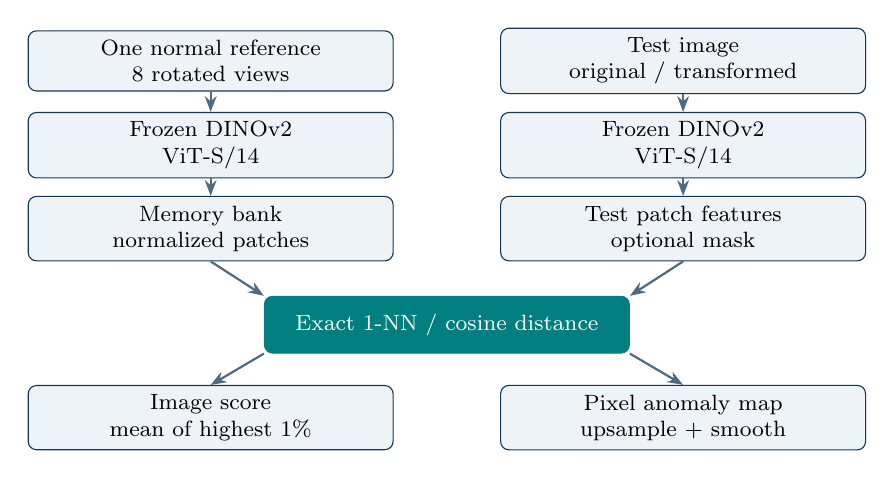
\begin{tikzpicture}[x=1cm,y=1cm, every node/.style={font=\footnotesize},box/.style={draw=navy,fill=pale,rounded corners=3pt,align=center,minimum height=.72cm,text width=4.4cm},matchbox/.style={box,fill=teal,text=white,draw=teal},a/.style={-{Stealth[length=2mm]},thick,draw=muted}]
\node[box] (r) at (-3,2) {One normal reference\\8 rotated views};
\node[box] (t) at (3,2) {Test image\\original / transformed};
\node[box] (e1) at (-3,.93) {Frozen DINOv2\\ViT-S/14};
\node[box] (e2) at (3,.93) {Frozen DINOv2\\ViT-S/14};
\node[box] (m) at (-3,-.13) {Memory bank\\normalized patches};
\node[box] (q) at (3,-.13) {Test patch features\\optional mask};
\node[matchbox,text width=4.4cm] (n) at (0,-1.35) {Exact 1-NN / cosine distance};
\node[box] (s) at (-3,-2.53) {Image score\\mean of highest 1\%};
\node[box] (p) at (3,-2.53) {Pixel anomaly map\\upsample + smooth};
\draw[a] (r)--(e1); \draw[a] (t)--(e2); \draw[a] (e1)--(m); \draw[a] (e2)--(q);
\draw[a] (m.south)--(n.north west); \draw[a] (q.south)--(n.north east);
\draw[a] (n.south west)--(s.north); \draw[a] (n.south east)--(p.north);
\end{tikzpicture}
\smallnote{Schematic of the thesis implementation. 448-pixel short edge; 14-pixel patches; 384-dimensional embeddings. No weight updates.}
\end{frame}

\begin{frame}{Experimental design: matched comparisons}
\begin{columns}[T,onlytextwidth]
\column{.45\textwidth}
{\Large\key{15 categories}}\par
\vspace{.12cm}
MVTec AD: 3,629 normal training images; 1,725 test images (467 normal, 1,258 defective).
\vspace{.25cm}
\begin{itemize}
\item One original normal image per run.
\item Three fixed reference choices per category.
\item Same test images and labels across conditions.
\end{itemize}
\column{.52\textwidth}
\small
\begin{tabular}{@{}lr@{}}
\toprule
Study & Evaluations\\\midrule
Clean baseline & 45\\
Test perturbations & 180\\
Four-bank ablation & 900\\
Frozen thresholds & 225\\
\bottomrule
\end{tabular}
\vspace{.35cm}
\begin{block}{Primary metrics}
Image AUROC: ranking\\
Pixel AUPRO: region overlap (FPR $\leq0.30$)
\end{block}
\end{columns}
\smallnote{Equal-weight means over categories and reference choices. These are matched evaluations, not independent samples.}
\end{frame}

\begin{frame}{RQ1: clean baseline matches published precision}
\begin{columns}[T,onlytextwidth]
\column{.46\textwidth}
\small
\begin{tabular}{@{}lrr@{}}
\toprule Metric (\%) & Paper & Ours\\\midrule
Image AUROC & 96.5 & \key{96.52}\\
Image AP & 98.1 & 98.14\\
Image F1-max & 96.0 & 95.96\\
Pixel AUROC & 96.3 & 96.26\\
Pixel F1-max & 57.9 & 57.94\\
Pixel AUPRO & 91.7 & \key{91.72}\\
\bottomrule
\end{tabular}
\vspace{.25cm}
\take{Strong ranking does not guarantee precise segmentation.}
\column{.51\textwidth}
\centering\fig{4.75cm}{07_baseline_category_comparison}
\smallnote{Thesis Figure 6.1; category means over three references. Restricted axis.}
\end{columns}
\smallnote{Published comparator: Damm et al., AnomalyDINO (WACV 2025), one-shot ViT-S/14 at 448 pixels.}
\end{frame}

\begin{frame}{RQ2: controlled changes isolate imaging sensitivity}
\begin{columns}[T,onlytextwidth]
\column{.47\textwidth}
\begin{block}{Brightness}
Multiply RGB intensities by 0.85 or 0.70.
\end{block}
\begin{block}{Gaussian blur}
Pillow radius 0.75 or 1.50 pixels after resizing.
\end{block}
\column{.5\textwidth}
\begin{block}{Paired design}
Original + four altered versions of the same test images.
\end{block}
\begin{itemize}
\item Keep normal references unchanged.
\item Same labels and masks.
\item Measure full pipeline, including optional foreground masking.
\end{itemize}
\end{columns}
\smallnote{Digital perturbations are controlled stress tests, not measurements of physical factory acquisition.}
\end{frame}

\begin{frame}{Blur is more damaging than digital darkening}
\begin{columns}[c,onlytextwidth]
\column{.66\textwidth}
\centering\fig{5.6cm}{08_robustness_macro_change}
\column{.31\textwidth}
{\large\bfseries Strong blur}\par\vspace{.25cm}
{\LARGE\color{red}\bfseries $-3.08$ pp}\par
Image AUROC\par\vspace{.45cm}
{\LARGE\color{red}\bfseries $-1.53$ pp}\par
Pixel AUPRO\par\vspace{.35cm}
Digital darkening had much smaller average effects.
\end{columns}
\smallnote{Thesis Figure 7.1. All 180 perturbation evaluations; changes relative to the archived clean baseline. pp = percentage points.}
\end{frame}

\begin{frame}{Frozen thresholds reveal rising false alarms}
\begin{columns}[c,onlytextwidth]
\column{.65\textwidth}
\centering\fig{5.45cm}{05_threshold_calibration}
\column{.32\textwidth}
{\Large\color{red}\bfseries 8.32\% $\to$ 20.34\%}\par
Baseline false-positive rate under strong blur.\par\vspace{.3cm}
\small
\begin{itemize}
\item 40 extra normal train images per category.
\item 45 frozen thresholds; 225 comparisons.
\item Baseline only.
\end{itemize}
\end{columns}
\smallnote{Thesis Figure 7.2. Retrospective calibration; additional normals are not reference-bank inputs. No measured augmented-bank FPR.}
\end{frame}

\begin{frame}{RQ3: augment the reference, not the model}
\begin{block}{Hypothesis}
Blurred reference features may cover acceptable changes in appearance without learning new model weights.
\end{block}
\centering
\begin{tabular}{@{}lccr@{}}
\toprule
Bank & Darkened views & Blurred views & Stored patches\\\midrule
Rotation-only & -- & -- & 8,192\\
Brightness & 0.85 & -- & 8,192\\
\key{Blur} & -- & 0.75 px & 8,192\\
Combined & 0.85 & 0.75 px & 8,192\\
\bottomrule
\end{tabular}
\vspace{.2cm}
\smallnote{Eight rotated original views are available in every bank. Combined pools separate transformed views. Equal cardinality controls storage, not total computational cost.}
\end{frame}

\begin{frame}{Fixed-budget blur augmentation improves image ranking}
\begin{columns}[c,onlytextwidth]
\column{.65\textwidth}
\centering\fig{5.45cm}{01_ablation_image_auroc}
\column{.32\textwidth}
{\small\bfseries Strong blur}\par
{\LARGE\key{94.98\%}}\par
vs. 93.44\% rotation-only\par\vspace{.3cm}
{\Large\key{+1.54 pp}}\par
Image AUROC\par\vspace{.25cm}
\small 900 matched evaluations; shared test features and masks across banks.
\end{columns}
\smallnote{Thesis Figure 8.1. Same-pipeline rotation-only comparator; restricted vertical axis.}
\end{frame}

\begin{frame}{Localization gains are smaller and less consistent}
\begin{columns}[c,onlytextwidth]
\column{.65\textwidth}
\centering\fig{5.35cm}{02_ablation_pixel_aupro}
\column{.32\textwidth}
{\Large\key{+0.16 pp}}\par
Strong-blur pixel AUPRO\par\vspace{.35cm}
{\Large\color{red}\bfseries $-0.10$ pp}\par
Clean pixel AUPRO\par\vspace{.3cm}
\small Better image ranking does not imply better defect localization.
\end{columns}
\smallnote{Thesis Figure 8.2. Same 8,192-patch budget for each bank; restricted axis.}
\end{frame}

\begin{frame}{Category variation matters}
\begin{columns}[T,onlytextwidth]
\column{.49\textwidth}
\centering\fig{4.6cm}{03_strong_blur_category_image}
\column{.49\textwidth}
\centering\fig{4.6cm}{04_strong_blur_category_pixel}
\end{columns}
\vspace{.12cm}
\small \key{13/15} categories improve in image AUROC; Transistor contributes +14.04 pp. Excluding it, mean gain remains +0.65 pp; median gain +0.27 pp. Pixel AUPRO improves in 8 categories and declines in 7.
\smallnote{Thesis Figures 8.3--8.4. Descriptive paired effects; no independent-sample significance claim.}
\end{frame}

\begin{frame}{What does blur do to the anomaly maps?}
\begin{columns}[c,onlytextwidth]
\column{.60\textwidth}
\centering\fig{6.35cm}{09_selected_blur_cases}
\column{.37\textwidth}
\begin{itemize}
\item Normal Transistor: score rises.
\item Defective Transistor, Screw and Cable: scores fall.
\item Selected extremes illustrate possible failure mechanisms, not their frequency.
\end{itemize}
\smallnote{Cyan contours denote ground truth; paired heatmaps share a row-level color scale.}
\end{columns}
\smallnote{Thesis Figure 9.1; original archived maps. MVTec AD image/mask derivatives, CC BY-NC-SA 4.0.}
\end{frame}

\begin{frame}{The scientific contribution and its boundaries}
\begin{columns}[T,onlytextwidth]
\column{.48\textwidth}
\begin{block}{What the evidence supports}
\begin{itemize}
\item Reproduced one-shot benchmark.
\item Matched robustness and frozen-threshold evaluation.
\item Controlled fixed-budget augmentation and documented trade-offs.
\end{itemize}
\end{block}
\column{.49\textwidth}
\begin{block}{What remains unverified}
\begin{itemize}
\item Real industrial acquisition shifts or other datasets.
\item Augmented-bank false-alarm reduction.
\item Independent full GPU replay of reorganized workflow.
\end{itemize}
\end{block}
\end{columns}
\smallnote{Three fixed reference choices share test sets; they are not independent statistical replicates.}
\end{frame}

\begin{frame}{Reproducibility: from raw records to thesis figures}
\begin{columns}[T,onlytextwidth]
\column{.54\textwidth}
\begin{itemize}
\item Pinned AnomalyDINO and DINOv2 fingerprints.
\item Reference identities and SHA-256 checksums.
\item Five numbered analysis notebooks; three public entry-point scripts.
\item Archived predictions and map reconstruction.
\end{itemize}
\column{.43\textwidth}
\begin{block}{Verified audit}
623 numerical table cells\\
9/9 experimental figure PDF hashes\\
58 archived report checksum entries
\end{block}
\small CPU analysis re-executed from a fresh clone; selected maps reconstructed from original archive.
\end{columns}
\vfill
\small\url{https://github.com/basharbd/msc-visual-anomaly-detection}
\end{frame}

\begin{frame}{Conclusion: blur-aware references help, within limits}
\begin{block}{RQ1}
Clean baseline: \key{96.52\% image AUROC}, 91.72\% pixel AUPRO.
\end{block}
\begin{block}{RQ2}
Strong blur: \alert{$-3.08$ pp} image AUROC; frozen-threshold FPR increases to 20.34\%.
\end{block}
\begin{block}{RQ3}
Blur augmentation: \key{+1.54 pp} image AUROC under strong blur at fixed cardinality; smaller localization gain.
\end{block}
\smallnote{Next: real imaging shifts, independent datasets, more reference choices and augmented-bank threshold calibration.}
\end{frame}

\begin{frame}[plain]
\vfill
\centering
{\color{teal}\Large\bfseries Thank you}\par
\vspace{.35cm}
{\Huge\bfseries Questions?}\par
\vspace{.65cm}
{\large Bashar Khaled Bdewi}\par
DTU Compute \quad | \quad MSc thesis defense\par
\vspace{.3cm}
\small\url{https://github.com/basharbd/msc-visual-anomaly-detection}
\vfill
\end{frame}

\appendix
\begin{frame}{Backup: patch scoring and localization}
\small
For unit-normalized test and memory embeddings, exact L2 search yields cosine distance:
\[
 a_i=\tfrac12\min_{v\in\mathcal M}\|\bar z_i-\bar v\|_2^2
\]
Masked test patches receive zero. If $N$ is the number of patches and $q=\max(1,\lfloor 0.01N\rfloor)$:
\[
 s(x)=\frac{1}{q}\sum_{j=1}^q a_{(j)},\qquad a_{(1)}\geq\cdots\geq a_{(N)}.
\]
Raw patch grids are resized to original image dimensions and smoothed with Gaussian $\sigma=4$ pixels. Cropped bottom/right margins are not separately restored.
\end{frame}

\begin{frame}{Backup: calibration and metric interpretation}
\begin{columns}[T,onlytextwidth]
\column{.48\textwidth}
\begin{block}{Frozen operating point}
40 extra normal training images per category, excluding the three reference images. Threshold = 39th smallest score; classify anomalous if score $>\tau$.
\end{block}
\column{.49\textwidth}
\begin{block}{Metric distinction}
AUROC: ranking across thresholds.\\
AUPRO: region overlap, normalized up to FPR 0.30.\\
F1-max: optimized threshold on evaluated scores, not deployment calibration.
\end{block}
\end{columns}
\smallnote{Nominal 5\% calibration tail does not guarantee 5\% FPR on shifted test images.}
\end{frame}

\begin{frame}{Backup: paired Bottle scores under strong blur}
\begin{columns}[c,onlytextwidth]
\column{.60\textwidth}
\centering\fig{5.75cm}{10_bottle_paired_scores}
\column{.37\textwidth}
\begin{itemize}
\item 83 test images, reference index 0.
\item 20 normal, 63 anomalous.
\item Above diagonal: higher score after blur.
\item Below diagonal: lower score after blur.
\end{itemize}
\end{columns}
\smallnote{Thesis Figure 9.2; full-precision paired archived scores.}
\end{frame}

\begin{frame}{Backup: archive parity and recovery}
\begin{itemize}
\item 444 matched ablation evaluations reused; 456 completed during bounded recovery.
\item All 225 rotation-only comparisons agree exactly in image AUROC, AP and F1-max.
\item Maximum pixel AUPRO difference: 0.001012 pp.
\item Two Screw strong-blur runs have localized raw-map differences (0.117 and 0.169); cause not established.
\item Bank cardinality fixed, but augmentation may increase preparation cost.
\end{itemize}
\smallnote{See thesis Section 8.5 and the repository parity audit for the full record.}
\end{frame}

\begin{frame}{Backup: core references}
\small
\begin{itemize}
\item Damm et al. \emph{AnomalyDINO: Boosting Patch-Based Few-Shot Anomaly Detection with DINOv2}. WACV, 2025.
\item Oquab et al. \emph{DINOv2: Learning Robust Visual Features without Supervision}. TMLR, 2024.
\item Bergmann et al. \emph{MVTec AD --- A Comprehensive Real-World Dataset for Unsupervised Anomaly Detection}. CVPR, 2019.
\item Jeong et al. \emph{WinCLIP: Zero-/Few-Shot Anomaly Classification and Segmentation}. CVPR, 2023.
\end{itemize}
\smallnote{Full bibliography in the thesis. Experimental plots use the identical canonical PDF exports from the notebooks.}
\end{frame}
\end{document}
